\setcounter{secnumdepth}{3} %para tener una profundidad más en las enumeraciones
\chapter{Implementaci\'on}
\label{cap:implementacion}
En el Capítulo 3 se abordó la descripción de la herramienta sin entrar en detalles de como estaba implementada, una visión general de lo que se iba a ofrecer, como la organización de los componentes, los tipos de daño o los diferentes tipos de actuadores. En este capítulo se va a tratar en profundidad la implementación de estos componentes, hablando de cómo funcionan, cómo se pueden personalizar y como los distintos componentes interactúan entre ellos.\\

La implementación de la herramienta puede encontrarse en el siguiente enlace: \href{https://github.com/CristinaMora/EnemyBehaviourFramework-2D.git}{https://github.com/CristinaMora/EnemyBehaviourFramework-2D.git}.



\section{Tecnología utilizada}
Este proyecto ha sido desarrollado íntegramente en Unity, mencionado en el Capítulo 2 de este trabajo, concretamente la versión 2022.3.18f1(LTS) del motor. Por consiguiente, no podemos garantizar su correcto funcionamiento en versiones previas. No obstante, la previsión de la herramienta es ofrecer el correcto funcionamiento en versiones posteriores, salvo modificaciones significativas en la API fundamental de Unity.\\

El motivo por el que se escoge Unity sobre los demás motores de videojuegos es esa accesibilidad que ha sido mencionada anteriormente que hace que resulte sencillo de utilizar por cualquier persona. \\

Se hará uso de otros elementos de Unity para llevar a cabo esta herramienta como el motor de físicas 2D o las herramientas que tiene el motor para ayudar al usuario a debuggear como puede ser Gizmos.
Unity funciona mediante una arquitectura por componentes, lo que es muy útil para que el programa sea modular, que pueda ser dividido en piezas más pequeñas y que estas piezas sean independientes.\\

La herramienta desarrollada en este proyecto tiene como objetivo facilitar la creación y configuración de enemigos en un entorno 2D dentro de Unity. Está diseñada como un plugin modular que permite a diseñadores y desarrolladores configurar enemigos sin necesidad de escribir código, mediante un sistema visual e intuitivo basado en prefabs y componentes reutilizables.\\

En el núcleo de esta arquitectura se encuentra un sistema basado en una Máquina de Estados Finita (FSM). Cada enemigo definirá su comportamiento con una FSM que gestiona su comportamiento, transiciones entre estados y reacciones ante el entorno. Los estados están compuestos por actuadores (actuators), que ejecutan acciones (como movimiento, ataque o generación de enemigos), y sensores, que detectan condiciones o eventos del entorno y disparan transiciones entre estados.\\

Los elementos que conforman esta arquitectura se organizan en varios niveles:
\begin{itemize}
	\item Estados: Definen el comportamiento que el enemigo adopta en un momento determinado.
	\item Sensores: Detectan eventos del entorno, como la presencia del jugador o colisiones.
	\item Actuadores: Ejecutan acciones concretas, como moverse, disparar o generar nuevos enemigos.
	\item Emisores de daño: Permiten que los enemigos inflijan daño a otras entidades.
\end{itemize}

La herramienta incluye también una serie de prefabs preconfigurados que facilitan el uso del sistema y permiten una rápida iteración por parte del diseñador. Estos prefabs agrupan configuraciones comunes de enemigos con distintos comportamientos, reduciendo el tiempo de prototipado y aumentando la reutilización del código.\\

En resumen, lo que se ha creado es una herramienta extensible compuesta por componentes modulares, basada en la arquitectura de componentes de Unity, que permite crear comportamientos complejos mediante una configuración visual, facilitando así su adopción por parte de usuarios con conocimientos limitados de programación.\\

A continuación se va a hacer una descripción específica de cada uno de los apartados implementados.


\section{Actuator}

Un actuator es el componente encargado de ejecutar una acción, por lo que para cada tipo de acción existirá un actuator que la represente.
La clase \texttt{Actuator} representa la clase base de la que heredarán todos los tipos de actuadores.
Esta clase abstracta contiene métodos para crear, destruir y actualizar cada actuador, así como un booleano que indica si el Actuador tiene la depuración activa o no.\\

\subsection{MovementActuator}
La clase \texttt{Movement Actuator} que hereda de \texttt{Actuator} se usa para todos aquellos actuadores que realizan una acción de movimiento. \\

\textbf{Parámetros de configuración}
\begin{itemize}
	\item (bool) \textbf{Is Accelerated}: Indica si el movimiento que se va a realizar tiene una velocidad constante (valor a false), o que por el contrario, la velocidad va a ir variando (valor a true).
	\item (\texttt{EasingFunction.Ease}) \textbf{Easing Function}: Función que define cómo varía el movimiento en el tiempo. Este parámetro solo se requiere si el movimiento es acelerado.
\end{itemize}

\subsubsection{HorizontalActuator}
\texttt{Horizontal Actuator} es un actuador que hereda de \texttt{Movement Actuator} y permite mover un objeto horizontalmente, ya sea a la izquierda o a la derecha, con diferentes configuraciones de velocidad y comportamientos tras una colisión.\\

\textbf{Parámetros de configuración}
\begin{itemize}
	\item (enum) \textbf{On Collision Reaction}: Reacción que va a tener el objeto al colisionar. Puede ser \textit{None} (sin reacción), \textit{Bounce} (rebota cambiando la dirección), o \textit{Destroy} (se destruye al colisionar).
	\item (\texttt{LayerMask}) \textbf{Layers To Collide}: En caso de querer algún tipo de reacción, especificar que máscara de capas que indica cuáles son las que utilizamos para colisionar con el objeto.
	\item (enum) \textbf{Direction}: Dirección inicial del movimiento. Puede ser \textit{Left} o \textit{Right}.
	\item (float) \textbf{Speed}: Velocidad del movimiento.
	\item (float) \textbf{Goal Speed}: Velocidad final del movimiento si éste es acelerado.
	\item (float) \textbf{Interpolation Time}: Duración en segundos que va desde la velocidad inicial a \textit{Goal Speed}.
	\item (bool) \textbf{Throw}: Indica si el movimiento es un lanzamiento, es decir, se lanzará inicialmente con una velocidad inicial y, en caso contrario, se aplicará constantemente una fuerza.
	\item (bool) \textbf{Follow Player}: Determina si la dirección del movimiento se ajusta automáticamente para acercarse al jugador.
\end{itemize}

\subsubsection{VerticalActuator}
\texttt{Vertical Actuator} permite mover un objeto verticalmente, ya sea arriba o abajo, con diferentes configuraciones de velocidad y comportamientos tras una colisión.\\

\textbf{Parámetros de configuración}
\begin{itemize}
	\item (enum) \textbf{On Collision Reaction}: Reacción que va a tener el objeto al colisionar. Puede ser \textit{None} (sin reacción), \textit{Bounce} (rebota cambiando la dirección), o \textit{Destroy} (se destruye al colisionar).
	\item (\texttt{LayerMask}) \textbf{Layers To Collide}: Máscara de capas que indica cuáles son las que utilizamos para colisionar con el objeto.
	\item (enum) \textbf{Direction}: Dirección inicial del movimiento. Puede ser \textit{Up} o \textit{Down}.
	\item (float) \textbf{Speed}: Velocidad del movimiento.
	\item (float) \textbf{Goal Speed}: Velocidad final del movimiento si éste es acelerado.
	\item (float) \textbf{Interpolation Time}: Duración en segundos que va desde la velocidad inicial a \textit{Goal Speed}.
	\item (bool) \textbf{Throw}: Indica si el movimiento es un lanzamiento, es decir, se lanzará inicialmente con una velocidad inicial y, en caso contrario, se aplicará constantemente una fuerza.
	\item (bool) \textbf{Follow Player}: Determina si la dirección del movimiento se ajusta automáticamente para acercarse al jugador.
\end{itemize}

\subsubsection{DirectionalActuator}
La clase \texttt{Directional Actuator} se usa para describir un movimiento en función de un ángulo y una velocidad.\\

\textbf{Parámetros de configuración}
\begin{itemize}
	\item (\texttt{LayerMask}) \textbf{Layers To Collide}: Capas con las que puede colisionar el objeto y activar reacciones.
	\item (float) \textbf{Speed}: Velocidad del movimiento.
	\item (float) \textbf{Goal Speed}: Velocidad final del movimiento si este es acelerado.
	\item (float) \textbf{Interpolation Time}: Duración en segundos que va desde la velocidad inicial a \textit{Goal Speed}.
	\item (float) \textbf{Angle}: Ángulo de dirección del movimiento, en grados, siéndo 0º un movimiento hacía la derecha. Los grados se suman en sentido antihorario.
	\item (bool) \textbf{Throw}: Indica si el movimiento es un lanzamiento, es decir, si está a true, se lanzará inicialmente con una velocidad inicial y, en caso contrario, se aplicará constantemente una fuerza.
	\item (enum) \textbf{On Collision Reaction}: Reacción que va a tener el objeto al colisionar. Puede ser \textit{None} (sin reacción), \textit{Bounce} (rebota cambiando la dirección), o \textit{Destroy} (se destruye al colisionar).
	\item (bool) \textbf{Aim Player}: Determina si el objeto calculará automáticamente el ángulo inicial para moverse en dirección al jugador.
\end{itemize}

\subsubsection{CircularActuator}
La clase \texttt{Circular Actuator} se usa para describir un movimiento circular alrededor de un punto.\\

\textbf{Parámetros de configuración}
\begin{itemize}
	\item (float) \textbf{Angular Speed}: Velocidad de giro en grados por segundo.
	\item (\texttt{Transform}) \textbf{Rotation Point Position}: Punto central de la circunferencia que describe el objeto.
	\item (float) \textbf{Max Angle}: Ángulo máximo de giro. Si el ángulo es \textit{360º} entonces describirá una circunferencia completa, si no, hará un movimiento en forma de péndulo con los grados indicados.
	\item (float) \textbf{Angular Acceleration}: Aceleración angular.
	\item (float) \textbf{Goal Angular Speed}: Velocidad angular que se quiere alcanzar si el objeto es acelerado.
	\item (bool) \textbf{Can Rotate}: Determina si el objeto rota sobre sí mismo siguiendo la trayectoria.
	\item (float)\textbf{ Interpolation Time}: Tiempo en segundos que tarda desde la velocidad inicial hasta la velocidad final, \textit{Goal Speed}.
	\item (bool) \textbf{Point Player}: Determina si el objeto se orienta automáticamente hacia el jugador.
\end{itemize}

\subsubsection{SplineFollowerActuator}
La clase \texttt{SplineFollowerActuator} se usa para describir un movimiento mediante curvas Splines de Unity. El Actuador sigue la curva pudiendo girar el objeto a su vez.\\

\textbf{Parámetros de configuración}
\begin{itemize}
	\item (float) \textbf{Speed}: Velocidad del movimiento.
	\item (float) \textbf{Goal Speed}: Velocidad final del movimiento si este es acelerado.
	\item (float) \textbf{Interpolation Time}: Duración en segundos que va desde la velocidad inicial a \textit{Goal Speed}.
	\item (\texttt{SplineContainer}) \textbf{Spline Container}: Objeto que define una trayectoria basada en una spline, como la descrita en la \autoref{act:splinefollower} y representada en la \autoref{fig:SplineFollowerActuator_Image}. Este componente permite establecer una serie de puntos de control conectados por curvas suaves, editables directamente en el editor de Unity. Además, el \texttt{SplineContainer} ofrece funciones para acceder a la curva en tiempo real, interpolar posiciones a lo largo del recorrido y orientar el objeto dinámicamente durante su desplazamiento.
	\item (enum) \textbf{Teleport To Closest Point}: Define cómo se ajusta el objeto a la spline al iniciarse el movimiento. Puede tener dos valores:
	\begin{itemize}
		\item \textbf{Move Enemy To Spline}: El enemigo se teletransporta a la spline.
		\item \textbf{Move Spline To Enemy}: La spline se desplaza para alinearse con la posición actual del objeto.
	\end{itemize}
\end{itemize}

\begin{figure}[t]
	\centering
	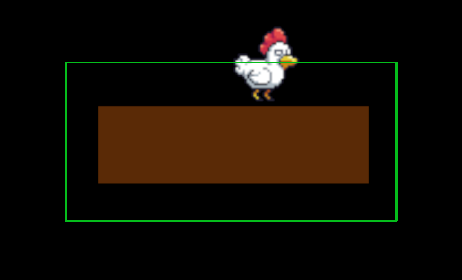
\includegraphics[width = 0.7\textwidth]{Imagenes/SplineFollowerActuator.png}
	\caption{Uso de Spline para definir el camino de un enemigo.}
	\label{fig:SplineFollowerActuator_Image}
\end{figure}

\subsubsection{MoveToAPointActuator}
La clase \texttt{Move To A Point Actuator} se usa para mover el objeto en dirección a un punto no actualizable. Puede ser a un punto concreto y seguir una lista de ellos o a puntos aleatorios dentro de un área (descripción completa en {\ref{sec:MoveToAPoint}}).\\
Dado que la clase tiene dos maneras de funcionar y dos configuraciones distintas, primero se abordarán los parámetros de configuración comunes entre ambas y luego los parámetros específicos de cada configuración.\\

\textbf{Parámetros de configuración comunes}
\begin{itemize} 
	\item (enum) \textbf{Mode}: Define si se va a seguir una ruta por puntos (\textit{Waypoint}) o si se escogen puntos aleatoriamente dentro de una zona (\textit{RandomArea}).
\end{itemize}	
\begin{figure}[t]
		\centering
		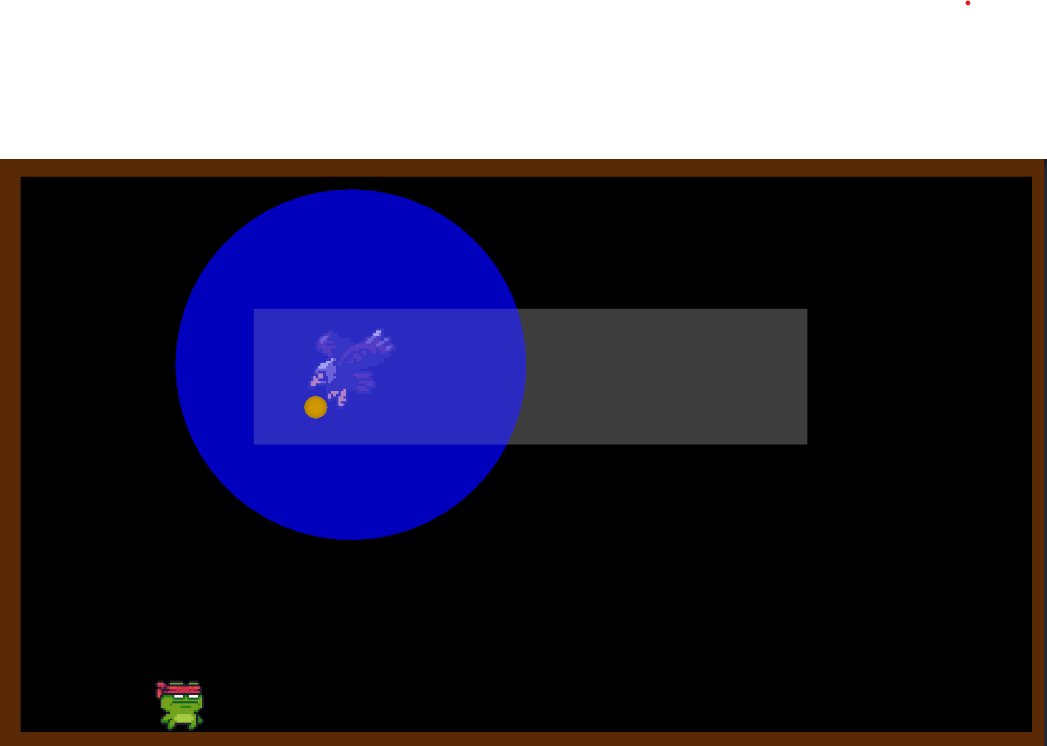
\includegraphics[width = 0.7\textwidth]{Imagenes/MoveToAPointRandomArea.png}
		\caption{Modo Random Area, se aprecia una zona azul (DistanceSensor), un rectángulo gris (zona donde aparecen nuevos puntos) y por último un punto amarillo (waypoint actual).}
		\label{fig:MoveToAPointRandomArea_Image}
\end{figure}
\textbf{Parámetros de configuración para Waypoint}
\begin{itemize} 	
	\item (bool) \textbf{Loop}: Determina si al finalizar los puntos volverá al primero y el movimiento se repetirá.
	\item (bool) \textbf{All Waypoints Have The Same Data}: Determina si todos los puntos usarán la misma configuración.
	\item (List<\texttt{WaypointData}>) \textbf{Waypoints Data}: Lista de puntos que el objeto debe seguir. En este caso el struct \texttt{WaypointData} está compuesto por:
	\begin{itemize} 	
		\item (\texttt{Transform}) \textbf{Waypoint Transform}: Posición a la que se debe de llegar.
		\item (float) \textbf{Time To Reach}: Tiempo estimado para alcanzar la posición deseada.
		\item (bool) \textbf{Is Accelerated}: Si se requiere aceleración.
		\item (\texttt{EasingFunction.Ease}) \textbf{Easing Function}: Función de aceleración que describe como varía la posición del objeto con respecto al tiempo, en caso de tratarse de un movimiento acelerado.
		\item (bool) \textbf{Should Stop}: Indica si debe detenerse al llegar.
		\item (float) \textbf{Stop Duration}: Tiempo que debe durar la parada en caso de existir.
	\end{itemize}
\end{itemize}

\textbf{Parámetros de configuración para RandomArea}
\begin{itemize} 	
	\item (\texttt{Collider2D}) \textbf{Random Area}: Zona dentro de la cual se moverá el objeto si está configurado como \textit{RandomArea}. 
	\item (float) \textbf{Time Between Random Points}: Tiempo necesario, en segundos, para ir de un punto aleatorio a otro.
\end{itemize}


\subsubsection{MoveToAnObjectActuator}
La clase \texttt{Move To An Object Actuator} se usa para mover el objeto en dirección a un punto actualizable, esto implica que si el punto se mueve, el objeto actualizará la trayectoria a la nueva posición.\\

\textbf{Parámetros de configuración}
\begin{itemize} 
	\item (\texttt{Transform}) \textbf{Object Transform}: Posición del objeto destino. No se necesita la referencia al objeto en sí, ya que lo único que se va a utilizar de éste es su posición.
	\item (float) \textbf{Time To Reach}: Tiempo necesario, en segundos, para llegar a la posición destino.
\end{itemize}

\subsection{SpawnerActuator}
La clase \texttt{SpawnerActuator} se usa para poder generar nuevos enemigos, pudiendo generar infinitos enemigos o un número definido de ellos cada cierto tiempo en un lugar predefinido.\\

\textbf{Parámetros de configuración}
\begin{itemize}
    \item (float) \textbf{Spawn Interval}: Intervalo de tiempo en segundos que tarda el objeto en volver a generar. 
    \item (bool) \textbf{Infinite Enemies}: Indica si se generarán enemigos indefinidamente. Si es verdadero, se crearán continuamente nuevos enemigos cada cierto tiempo indicado por \textit{Spawn Interval}. Si es falso, el número de spawns estará limitado por \texttt{Number of Times To Spawn}.
    \item (int) \textbf{Number Of Times To Spawn}: Número total de veces que se permitirá hacer spawn, si no es infinito.
    \item (List<\texttt{SpawnInfo}>) \textbf{Spawn Points}: Lista de elementos de tipo \texttt{Spawn Info}, clase compuesta por:
    \begin{itemize} 
	\item (\texttt{GameObject}) \textbf{Prefab To Spawn}: Objeto a instanciar.
	\item (\texttt{Transform}) \textbf{Spawn Point}: Punto de aparición del objeto.
    \end{itemize}
    Esta lista está diseñada para poder crear distintos tipos de enemigos o en varios sitios a la vez, dando así más flexibilidad.
\end{itemize}


\section{Sensor}

La clase \texttt{Sensor} actúa como clase base para todos los sensores de la herramienta. Implementa una arquitectura basada en el patrón observador (observer), en la que cualquier componente interesado puede registrarse para ser notificado cuando el sensor se active.

Cada sensor contiene una variable de tipo \texttt{Action<Sensor>} que alberga una lista de funciones (callbacks) a ejecutar cuando se detecta una condición específica. Estas funciones pueden ser proporcionadas por otros componentes, como por ejemplo una transición que deba activarse tras la detección.

Para garantizar una interfaz unificada, las funciones que se registren como oyentes deben aceptar un único parámetro de tipo \texttt{Sensor}. Esto permite que, al activar el sensor, se le pueda pasar una referencia a sí mismo, facilitando que el componente suscrito acceda a su información contextual si lo necesita.

Este enfoque permite una arquitectura desacoplada y extensible, donde los sensores no necesitan conocer directamente qué componentes responderán a su activación, simplemente notifican a todos los suscriptores registrados.

Además, la implementación del sistema de eventos incluye un contador de suscriptores, que permite llevar un control sobre cuántos componentes están actualmente registrados. Esta medida ayuda a evitar errores en tiempo de ejecución relacionados con notificaciones no deseadas o fugas de memoria.

Cualquier clase que herede de \texttt{Sensor} tendrá la posibilidad de modificar tres funciones relativas a la lógica del sensor:

\begin{itemize}
	\item \textit{StartSensor}: Función que se encarga de activar el sensor para que se pueda comenzar a captar información y, en caso de querer un tiempo de espera al inicio de la activación, se crea el \textit{timer} correspondiente.
	\item \textit{UpdateSensor}: Función llamada en cada bucle y encargada de actualizar el tiempo que queda por esperar en caso de que el \textit{timer} no haya acabado.
	\item \textit{StopSensor}: Función que desactiva el sensor.
\end{itemize}
Estas funciones gestionan el estado interno del sensor. Una de las variables indica si el sensor se encuentra activo o inactivo, mientras que otra se utiliza para facilitar la depuración, mostrando información útil sobre su estado actual.\\

\textbf{Parámetros de configuración}
\begin{itemize}
	\item (float) \textbf{Start Detecting Time}: Tiempo que necesitará el sensor para encenderse al entrar en el estado que lo alberga. Si el sensor no está encendido se considera que está apagado y su funcionalidad quedará suspendida hasta que esté encendido.
\end{itemize}

A continuación se enumerarán y explicarán los tipos de sensores incluidos en la herramienta.\\

\subsection{AreaSensor}

\texttt{AreaSensor} representa un tipo de sensor espacial que detecta la presencia de un objeto objetivo dentro de una zona delimitada (\autoref{fig:AreaSensor_Image}). Está pensado para funcionar con zonas de activación, por lo que requiere que el objeto que lo contiene tenga un componente \texttt{Collider2D}.\\

La detección se realiza mediante los métodos \textit{OnTriggerEnter/Stay/Exit2D} provistos por \textit{Unity}. 
El primero detecta la entrada del objetivo en la zona, mientras que el segundo permite capturar situaciones en las que el objetivo ya se encuentra dentro del área al momento de encenderse el sensor. Esto evita perder eventos relevantes si la detección no estaba habilitada previamente.\\

\textbf{Parámetros de configuración}
\begin{itemize}
	\item (\texttt{GameObject}) \textbf{Target}: Objeto que se quiere detectar dentro de la zona delimitada por el Collider2D.
\end{itemize}

\begin{figure}[t]
		\centering
		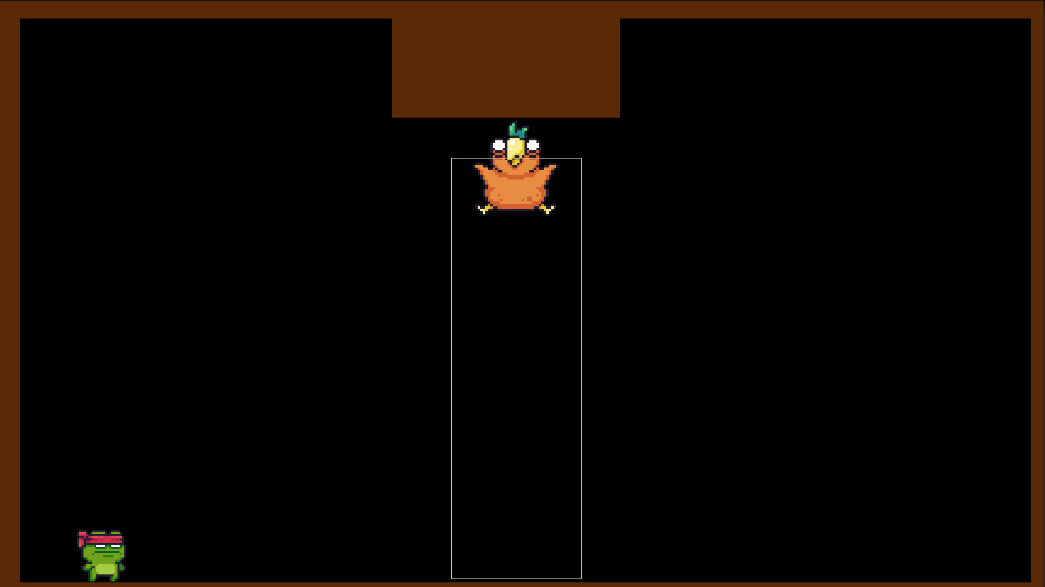
\includegraphics[width = 0.7\textwidth]{Imagenes/AreaSensor_Image.png}
		\caption{AreaSensor utilizado para enemigo que cae al detectar al jugador.}
		\label{fig:AreaSensor_Image}
\end{figure}
\subsection{CollisionSensor}
\texttt{CollisionSensor} es el sensor encargado de detectar colisiones entre el objeto que lo contiene y un conjunto específico de objetos definidos mediante una \texttt{LayerMask} de Unity. Al igual que el \texttt{AreaSensor}, este sensor requiere obligatoriamente la presencia de un componente \texttt{Collider2D} en el objeto. Para garantizarlo, se utiliza la anotación correspondiente en Unity que fuerza su inclusión automáticamente.\\

La detección de colisiones se realiza mediante los métodos \textit{OnCollisionEnter2D} y \textit{OnCollisionStay2D}. Este último es necesario para cubrir casos en los que la colisión ya se está produciendo cuando el sensor se enciende: si se utilizara únicamente \textit{OnCollisionEnter2D}, dichas situaciones no serían detectadas. Para que la colisión sea válida, es importante que ninguno de los dos objetos involucrados debe ser trigger.


\textbf{Parámetros de configuración}
\begin{itemize}
	\item (\texttt{LayerMask}) \textbf{Layers To Collide}: Máscara de capas físicas que, en caso de colisión, activarán el sensor.
\end{itemize}


\subsection{DistanceSensor}

\texttt{DistanceSensor} es el sensor utilizado para medir la distancia entre dos puntos. La distancia se medirá tomando de referencia las posiciones de sendos objetos, uno de ellos el que posee este componente y el otro el objetivo de la medición.\\

El funcionamiento del sensor dependerá del valor asignado a la variable \textit{Distance Type}, la cual es de un tipo enumerado \textit{TypeOfDistance} que especifica la manera en que se calculará la distancia. Según el valor de esta variable, se requerirán distintos parámetros o configuraciones, aunque varios valores de configuración seguirán siendo necesarios independientemente de \textit{Distance Type}.\\

\textbf{Parámetros de configuración comunes}
\begin{itemize}
	\item (enum) \textbf{Distance Type}: Tipo enumerado que determinará de qué manera se mide la distancia y qué variables se necesitarán para medirla.
	\item (enum) \textbf{Detection Condition}: Tipo enumerado que determina si el sensor se activa cuando el objetivo está dentro de esa distancia o cuando está fuera de la misma.
	\item (\texttt{GameObject})\textbf{ Target}: Entidad con la que se mide la distancia.
\end{itemize}

A continuación se especificarán los valores que puede tomar el enumerado \textit{TypeOfDistance}, sus usos y las variables específicas necesarias en cada caso.\\

\textbf{Valores de \textit{TypeOfDistance}}

\begin{itemize}
	\item \textit{Magnitude}

Configuración utilizada cuando se quiere medir la distancia como magnitud. La representación gráfica de esta forma de medir la distancia es un círculo, como se muestra en la \autoref{fig:DistanceSensor_Magnitude}.\\
Dependiendo del valor de la variable \textit{Detection Condition}, el sensor se activará si el objeto objetivo está dentro o fuera del círculo.
\begin{figure}[t]
	\centering
	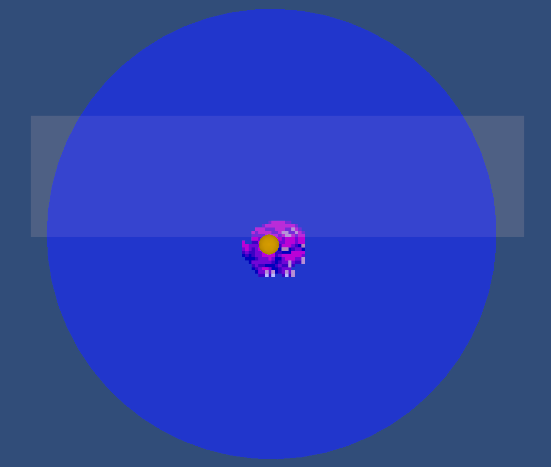
\includegraphics[width = 0.7\textwidth]{Imagenes/DistanceSensorMagnitude.png}
	\caption{Medición de distancia a través de la magnitud.}
	\label{fig:DistanceSensor_Magnitude}
\end{figure}

\textbf{Parámetros de configuración}
	\begin{itemize}
	        \item (float) \textbf{Detection Distance}: Distancia necesaria para que el sensor se active.
	 \end{itemize}

	\item \textit{Single Axis}

Con el tipo de medida \textit{Single Axis} se mide la distancia entre ambos objetos, pero solo en uno de los dos ejes: X o Y.\\
En la \autoref{fig:SingleAxis_Image} vemos un ejemplo de como luce la medición en el eje X.\\

\begin{figure}[t]
		\centering
		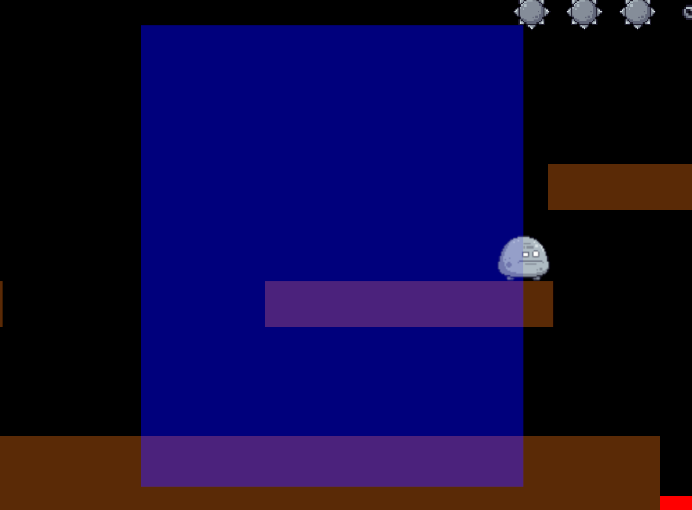
\includegraphics[width = 0.7\textwidth]{Imagenes/SingleAxis_Image.png}
		\caption{Medición de distancia en el eje X en su lado negativo.}
		\label{fig:SingleAxis_Image}
\end{figure}
\textbf{Parámetros de configuración}
	\begin{itemize}
	        \item (float) \textbf{Detection Distance}: Distancia necesaria para que el sensor se active.
	        \item (enum) \textbf{Axis}: Da opciones para escoger cuál de los dos ejes se va a medir, si X o Y.
	        \item (enum) \textbf{Detection Sides}: Permite elegir si se quiere medir la distancia a ambos lados del eje, en el lado positivo o en el lado negativo.
	 \end{itemize}
\end{itemize}

\subsection{TimeSensor}

Sensor encargado de activarse cuando pasa un tiempo determinado desde su activación. En caso de ajustar que el sensor necesitará un tiempo para encenderse, primero se procederá a medir tal tiempo y, cuando este llegue a su fin, se medirá el tiempo de activación propio del sensor.\\

\textbf{Parámetros de configuración}
	\begin{itemize}
	        \item (float) \textbf{Detection Time}: Tiempo necesario, medido en segundos, para que el sensor se active.
	 \end{itemize}

\section{Damage}

En esta sección se abordará el como se gestiona todo lo relacionado con el daño a través de, principalmente, dos componentes: \texttt{DamageEmitter} y \texttt{DamageSensor}.

\subsection{DamageEmitter}
Para que una entidad pueda emitir daño, debe tener adjunto el componente \texttt{DamageEmitter}.\\
Este componente no implementa funcionalidad adicional en su propio componente, sino que actúa como una señal para el \texttt{DamageSensor}, que será explicado en el siguiente apartado. La detección de daño por parte del sensor depende de que el objeto con el que colisiona tenga este componente adjunto.\\

La manera en la que \texttt{DamageEmitter} reporta daño dependerá de un tipo enumerado llamado \texttt{DamageType}.\\
Como valores de configuración comunes para todas las configuraciones disponibles encontramos:\\

\textbf{Parámetros de configuración comunes}
\begin{itemize}
	\item (bool) \textbf{Active From Start}: En caso de que esté desactivado, no se reportará daño a no ser que el \texttt{DamageEmitter} esté incluido en un estado.
	\item (enum) \textbf{Damage Type}: Diferentes formas de producir daño a las entidades que tengan \texttt{DamageSensor}.
\end{itemize}

A continuación se concretarán los valores que puede tomar el enumerado \texttt{DamageType}, cómo funciona cada tipo de daño y qué otros valores de configuración serán necesarios.\\

\textbf{Valores de \textit{DamageType}}

\begin{itemize}
	\item \textit{Instant}
Tipo de daño que se aplica una vez producido el contacto y que no se va a volver a aplicar hasta que ese contacto no haya finalizado y se dé uno nuevo.\\

\textbf{Parámetros de configuración}
	\begin{itemize}
	        \item (bool) \textbf{Destroy After Doing Damage}: Booleano que determina si el objeto es destruido al reportar daño.
	        \item (bool) \textbf{Instant Kill}: Determina si la entidad que reporta daño elimina a su objetivo instantáneamente.
	        \item (float) \textbf{Damage Amount}: En caso de no eliminar instantáneamente al objetivo, se especificará la cantidad de daño que se hará.
	 \end{itemize}
	\item \textit{Permanence}
El daño de permanencia es aquel que produce constantemente una entidad cada cierto tiempo. Este daño se producirá mientras dure la colisión o, en caso de que sea un trigger, la superposición.\\

\textbf{Parámetros de configuración}
	\begin{itemize}
	        \item (float) \textbf{Damage Amount}: Cantidad de daño administrada cada vez.
	        \item (float) \textbf{Damage Cooldown}: Tiempo necesario para administrar daño de nuevo, medido en segundos.
	\end{itemize}

	\item \textit{Residual}
El daño residual es aquel que produce una cantidad de daño instantáneo y, tras esto, produce un número determinado de aplicaciones de otra cantidad de daño cada cierto tiempo.\\

\textbf{Parámetros de configuración}
	\begin{itemize}
	        \item (bool) \textbf{Destroy After Doing Damage}: Booleano que determina si el objeto es destruido al reportar el daño instantáneo.
	        \item (float) \textbf{Instant Damage Amount}: Cantidad de daño administrada cuando se produce el contacto.
	        \item (float) \textbf{Residual Damage Amount}: Cantidad de daño administrada por cada aplicación de daño residual.
	        \item (float) \textbf{Damage Cooldown}: Tiempo entre aplicaciones de daño residual, medido en segundos.
	        \item (int) \textbf{Number Of Applications}: Número de veces que se aplicará el daño residual.
	\end{itemize}
\end{itemize}
\subsection{DamageSensor}

\texttt{DamageSensor} es un tipo de sensor que detecta las colisiones y entradas en el área de un objeto que emite daño. Este sensor está diseñado para funcionar tanto con colisiones como con triggers. Requiere que el objeto al que se le asigne tenga un componente \texttt{Collider2D}.\\

La funcionalidad de este sensor es doble. Además de activar transiciones, se utiliza para gestionar la lógica del componente \texttt{Life}. En caso de colisión, y bajo ciertas condiciones, como colisionar con un objeto que tenga el componente \texttt{DamageEmitter}, el sensor se activa. Luego, desde el componente \texttt{Life}, se gestiona qué hacer en función de las características del \texttt{DamageEmitter}.\\

Dado que \texttt{Life} es un componente utilizado para contextualizar la herramienta, pero no necesariamente el único componente de vida posible, \texttt{DamageSensor} puede utilizarse para crear nuevos componentes de vida con distintas características, separando así la funcionalidad de ambos componentes.\\

El sensor puede ser configurado para que se active desde el inicio mediante el atributo \textit{Active From Start}, lo que permite que el sensor sea útil en caso de que no se quiera que el sensor esté implicado en ninguna transición, pero sí en el sistema de gestión de salud.\\

El sensor detecta las entradas y salidas de objetos mediante los métodos \textit{OnTriggerEnter2D}, \textit{OnTriggerExit2D}, \textit{OnCollisionEnter2D} y \textit{OnCollisionExit2D}. Este control será necesario para gestionar los distintos tipos de daños que serán abordados más adelante.\\

\textbf{Parámetros de configuración}
\begin{itemize}
	\item (bool) \textbf{Active From Start}: Si es verdadero, el \textit{DamageSensor} no tendrá por qué ser incluido en ninguna transición para que este se considere activo.
\end{itemize}

\section {Máquina de Estados Finita}

El comportamiento de la entidad estará encapsulado en una Máquina de Estados Finita, cuya única funcionalidad es la de gestionar el estado actual, comprobar que no ha habido ningún cambio de estado y, en caso de haberlo, manejar el cambio. Esta comprobación se hará al finalizar la actualización del estado actual (en el \texttt{LateUpdate}) para así evitar problemas con cambiar de estado en medio de un bucle sin terminar.\\

\textbf{Valores de configuración}
\begin{itemize}
	\item (\texttt{State}) \textbf{Initial State}: Estado inicial de la Máquina de Estados Finita.
\end{itemize}

\subsection{Transition}
Esta clase representa una transición de estado. Está compuesta por un sensor y un estado objetivo.Si el sensor se activa, la entidad cambiará automáticamente al estado especificado.\\

\textbf{Parámetros de configuración}
\begin{itemize}
	\item (\texttt{Sensor}) \textbf{Sensor}: Sensor encargado de detectar el evento que hará que se produzca el cambio de estado.
	\item (\texttt{State}) \textbf{Target State}: Estado de destino de la transición.
\end{itemize}

\subsection{State}

La clase \texttt{State} representa un estado de comportamiento de un enemigo. Para ello gestiona dos elementos fundamentales: \texttt{Actuators} y \texttt{Sensors}.\\


\textbf{Parámetros de configuración}
\begin{itemize}
	\item (List<\texttt{Actuator}>) \textbf{Actuator List}: Lista de Actuators que son actualizados en cada bucle y representan acciones.
	\item (List<\texttt{Transition}>) \textbf{Transition List}: Lista de Tansitions que pueden ser activadas.
	\item (List<\texttt{DamageEmitter}>) \textbf{Damage Emitter in State}: Lista de DamageEmitter activos en el estado
	\item (bool) \textbf{Debug State}: Booleano utilizado para indicar si se quiere que los Actuators en \textit{Actuator List} y Sensores en \textit{Transition List} muestren información a través del Gizmos.
\end{itemize}

En la \autoref{fig:State_Image} vemos como se distribuyen los parámetros en el inspector.\\

Cuando se produce un cambio de estado, todos los actuadores y sensores se detienen, y los sensores se desuscriben de todas las transiciones a los que estuvieran vinculados.\\
\begin{figure}[t]
		\centering
		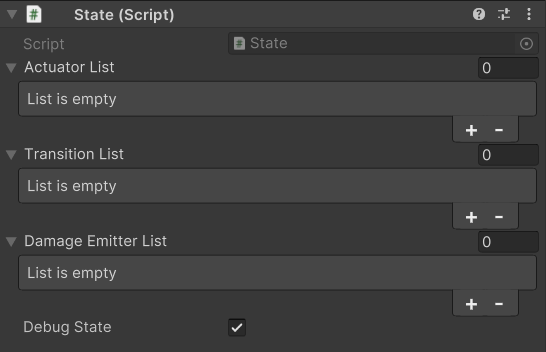
\includegraphics[width = 0.7\textwidth]{Imagenes/State.png}
		\caption{Distribución del inspector de clase \texttt{State}.}
		\label{fig:State_Image}
\end{figure}
\section{Animator Manager} \label{sec:animation}
La clase \texttt{AnimatorManager} se encarga de gestionar las animaciones de cada enemigo en función del movimiento, es decir, de los actuadores que estén activos.\\

\textbf{Parámetros de configuración}
\begin{itemize}
	\item (bool) \textbf{Can Flip X}: Indica si el sprite puede voltearse horizontalmente.
	\item (bool) \textbf{Can Flip Y}: Indica si el sprite puede voltearse verticalmente. 
	\item (\texttt{SpriteRender}) \textbf{Sprite Render}: Referencia al Sprite Render del propio objeto.
\end{itemize}

Durante la ejecución del juego, se monitoriza constantemente la velocidad del objeto mediante su componente \texttt{Rigidbody2D}. Esta información se utiliza para actualizar tres parámetros del \texttt{AnimatorManager}: \textit{XSpeed}, \textit{YSpeed} y \textit{RotationSpeed}. Estos parámetros permiten que el sistema de animaciones adapte en tiempo real la apariencia del personaje según su movimiento: por ejemplo, una animación de correr hacia la derecha cuando la velocidad en el eje X es positiva. Además, si el enemigo cambia de dirección (por ejemplo, pasa de moverse a la izquierda a hacerlo a la derecha), su sprite puede rotarse automáticamente para mantener la coherencia visual. Este comportamiento solo se aplica si se han activado previamente unos booleanos de configuración que permiten dicha rotación.

Cuando el enemigo recibe daño o muere, se activan los triggers \textit{Damage} y \textit{Die} respectivamente, lo que lanza las animaciones correspondientes. En el caso de la muerte, el objeto se destruye automáticamente una vez finaliza la animación. 

Por otro lado, se han definido varios parámetros y funciones que permiten controlar su comportamiento:
\begin{itemize}
	\item El parámetro \textit{Follow} (de tipo bool) indica si el enemigo debe seguir a otro objeto, normalmente el jugador.
	\item La función \textit{ChangeState} permite modificar el estado actual de la máquina de estados finita (FSM) del enemigo. Este cambio puede provocar una transición de animación o modificar su comportamiento.
	\item El trigger \textit{Spawn} se activa al instanciar el enemigo en la escena. Permite reproducir una animación de aparición o ejecutar lógica específica asociada a su entrada en el juego.
\end{itemize}

\textbf{Parámetros requeridos en el Animator}
Para sincronizar el comportamiento del enemigo con sus animaciones, se ha configurado un \texttt{Animator Controller} que utiliza los siguientes parámetros:
\begin{itemize}
	\item \textbf{Triggers}: \textit{Die}, \textit{Damage}, \textit{Spawn}, \textit{ChangeState}. Se activan para lanzar animaciones específicas cuando ocurren eventos clave (por ejemplo, recibir daño o morir).
	\item \textbf{Bools}: \textit{Left}, \textit{Right}, \textit{Up}, \textit{Down}, \textit{Follow}, \textit{Rotating}. Indican direcciones, estados o comportamientos que influyen en las transiciones de animación.
	\item \textbf{Floats}: \textit{XSpeed}, \textit{YSpeed}, \textit{RotationSpeed}. Permiten animar al enemigo en función de su velocidad de movimiento o rotación.
\end{itemize}

Para centralizar la gestión de las animaciones, se ha creado un controlador personalizado (\autoref{fig:AnimatorController_Image}), del tipo \texttt{Animator Controller}. Este actúa como una máquina de estados de animación, donde cada estado representa una animación (como caminar, aparecer, recibir daño, etc.), y las transiciones entre estados se controlan mediante los parámetros antes mencionados.Este enfoque facilita la integración entre la lógica del enemigo (programación) y su representación visual (animación).
\begin{figure}[t]
		\centering
		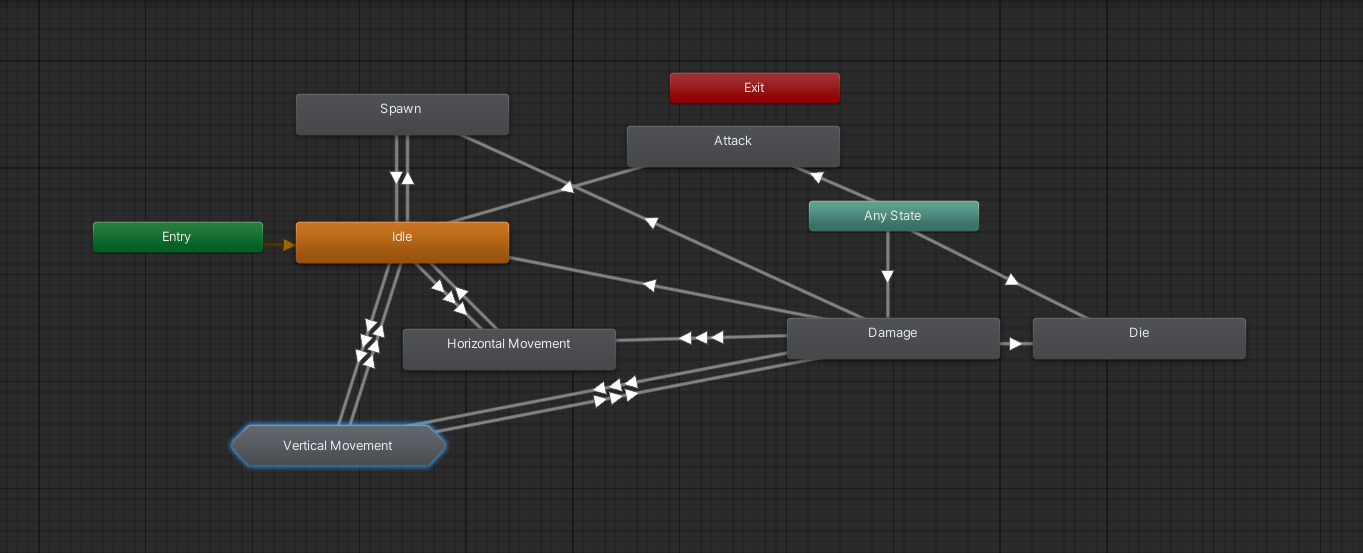
\includegraphics[width = 0.7\textwidth]{Imagenes/AnimatorController.png}
		\caption{AnimatorController con sus estados y transiciones.}
		\label{fig:AnimatorController_Image}
\end{figure}
\section{Jugador}

Como ayuda a la implementación, se han creado una serie de componentes auxiliares que dan funcionalidades básicas a todos los juegos y que, por tanto, eran esenciales para una implementación lógica. Esta sección y las siguientes estarán enfocadas en la explicación de estos elementos.\\
A la hora de implementar el movimiento del jugador usamos de base la implementación usada por el canal de YouTube \textit{Mix and Jam} en su interpretación del videojuego \textit{Celeste}\footnote{\url{https://www.youtube.com/watch?v=STyY26a_dPY}}.

\subsection{PlayerMovement}

La clase \textit{PlayerMovement} actúa como el controlador del jugador. Su función principal es gestionar la entrada del usuario y, en consecuencia, mover al personaje. Además, si el jugador se encuentra en el suelo y se presiona la tecla de salto, la clase se encarga de ejecutar el salto.
Asimismo, maneja una situación particular en la que el jugador queda suspendido en el aire mientras se mueve hacia una pared. Si este caso no se contempla, la fuerza ejercida en el eje X puede anular la del eje Y, haciendo que el personaje quede inmóvil en una posición poco natural. Para evitar este comportamiento, si el jugador está en el aire y colisiona lateralmente con una superficie, se le fuerza a deslizarse a lo largo de esta con una velocidad constante.
Esta clase permite modificar ciertos valores como la velocidad de movimiento, la potencia de salto o la velocidad con la que el jugador se desliza por las superficies anteriormente mencionadas.\\

\textbf{Valores de configuración}
\begin{itemize}
	\item (float) \textbf{Speed}: Velocidad constante a la que se moverá el jugador.
	\item (float) \textbf{Jump Force}: Fuerza aplicada al saltar
	\item (float) \textbf{Slide Speed}: Velocidad aplicada en el eje Y cuando el jugador está en el aire y colisiona lateralmente con una superficie.
\end{itemize}

\subsection{PlayerCollisionDetection}

Este componente se encarga de detectar las colisiones del jugador. Para ello, se ajustan tres cajas de colisión (\autoref{fig:Player_Coll_Detector}): una en cada lado y otra para detectar el contacto con el suelo. Las cajas no detectan realmente colisiones, sino que comprueban si estas se superponen con alguna entidad de las capas especificadas con el método \texttt{Physics2D.OverlapBox()}.\\

\textit{PlayerCollisionDetection} será usado por \textit{PlayerMovement} para gestionar acciones como determinar cuándo el jugador debe deslizarse por una superficie o cuándo puede saltar.\\

\begin{figure}[t]
	\centering
	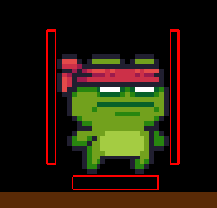
\includegraphics[width = 0.7\textwidth]{Imagenes/CollDetector.png}
	\caption{Representación de las cajas de detección de colisiones del jugador}
	\label{fig:Player_Coll_Detector}
\end{figure}

\textbf{Valores de configuración}
\begin{itemize}
	\item (bool) \textbf{ Debug Boxes}: En caso de que esta variable sea true, las cajas definidas por los campos que serán presentados a continuación serán representadas en pantalla con color rojo.
	\item (\texttt{LayerMask})  \textbf{Detection Layers}: Capas que serán tomadas en cuenta para detectar si el jugador está en el suelo o en contacto con una pared cuando está en el aire. En este caso se querrá especificar la capa que albergue a los objetos estáticos que conforman el mundo, por ejemplo \textit{World}.
	\item (\texttt{Vector2}) \textbf{Bottom/Right/Left Size}: Tamaño de las cajas.
	\item (\texttt{Vector2}) \textbf{Bottom/Right/Left Offsets}: Valores usados para reposicionar las cajas para que estén en el lugar considerado por el usuario, idealmente en los bordes del objeto.
\end{itemize}

\subsection{PlayerJump}

Para que el salto se ajuste más al estándar de los juegos de plataformas 2D, este script mejora la sensación de salto para que el personaje caiga más rápido, evitando una sensación de flotación. Además, permite realizar saltos más pequeños si el jugador suelta el botón antes.\\

Para lograrlo, el componente ajusta dos multiplicadores: uno que incrementa la gravedad cuando el jugador está cayendo y otro que reduce la altura del salto cuando este es interrumpido antes de tiempo.\\

\textbf{Parámetros de configuración}
\begin{itemize}
	\item (float) \textbf{Fall Multiplier}: Multiplicador que aumenta la gravedad cuando el personaje está cayendo, hace que el personaje caiga más rápido, dándole más peso y realismo al salto.
	\item (float) \textbf{Low Jump Multiplier}: Multiplicador que aumenta la gravedad cuando el jugador suelta el botón de salto antes de llegar al punto más alto del salto, haciendo que se puedan hacer saltos cortos, dando más control del movimiento al jugador.
\end{itemize}

\subsection{Life}

Se ha implementado una clase Life que gestiona los puntos de salud del objeto al que está adjunto y que se encarga de eliminar el objeto en el caso de que su vida llegue a cero. El componente pedirá al usuario un valor inicial para los puntos de vida del objeto y un valor máximo al que puede llegar la vida, para que esta sea limitada en caso de que se quiera implementar un sistema de recuperación de vida.\\

Este componente está estrechamente ligado al \textit{DamageSensor} que detecta si ha habido una colisión con un objeto que aplique daño. Esta relación es necesaria ya que, para que se detecte el daño que decrementa la salud del objeto, se necesita este sensor, por lo que al añadir un componente \textit{Life} se añadirá este sensor automáticamente.\\

\textit{Life} diferencia entre enemigos y el jugador; en caso de que el componente esté adjunto al jugador, se deberá marcar en la opción \textit{EntityType} y el componente requerirá que se le dé la referencia a un texto del \textit{Canvas} donde se escribirá la vida actual del jugador.\\

\textbf{Parámetros de configuración}
\begin{itemize}
	\item (enum) \textbf{Entity Type}: Enumerado usado para diferenciar entre jugador y enemigos.
	\item (float) \textbf{Initial Life}: Cantidad de vida con la que inicia la entidad.
	\item (float) \textbf{Max Life}: Cantidad de vida máxima a la que puede llegar la entidad.
	\item (string) \textbf{Text Name}: En caso de ser el jugador, se pedirá un texto que precederá a los puntos de vida del jugador.
	\item (\texttt{TextMeshProUGUI}) \textbf{Life Text}: Objeto del Canvas usado para representar los puntos de vida actuales del jugador.
\end{itemize}

\subsection{PlayerDistanceAttack}

Componente encargado de representar un posible ataque a distancia del jugador. El ataque se activará con el clic izquierdo del ratón, lo que instanciará el prefab \textit{Bullet Prefab} en la posición del jugador (será importante que el objeto instanciado no pueda colisionar con el jugador, por lo que se proporciona con la herramienta un prefab llamado \textit{PlayerBullet} que ya cumple con esta característica), el cual deberá albergar el comportamiento de una bala. La dirección que tomará la bala será aquella en la que se encuentre el cursor del ratón en el momento del clic.\\

Para evitar que el jugador pueda disparar sin restricción, se ha introducido un tiempo de espera entre disparos.\\

\textbf{Parámetros de configuración}
\begin{itemize}
	\item (\texttt{GameObject}) \textbf{Bullet Prefab}: Objeto que se instancia en la posición del jugador al hacer clic.
	\item (float) \textbf{Shooting Cooldown}: Tiempo necesario (en segundos) antes de poder disparar nuevamente.
\end{itemize}

\section {Distribución de la herramienta}

El Framework será distribuido a través de un archivo \textit{.unitypackage} descargable desde el repositorio de la herramienta.\\

Una vez descargado, el usuario podrá acceder a todo el contenido distribuido, que se detalla a continuación:\\
\begin{itemize}
\item \textbf{Animations:} Carpeta donde se encuentran tanto los \textit{sprites} usados como los \texttt{AnimatorController} creados para los enemigos de ejemplo.
\item \textbf{Materials:} En este directorio se encuentran materiales usados en la herramienta y el \texttt{Physic Material 2D} usado en algunos enemigos para mejorar su interacción con el jugador.
\item \textbf{Prefabs:} En la carpeta de \textit{Prefabs} se encuentran todos los \textit{prefabs} utilizados en la herramienta. También se encuentra el prefab \textit{BaseEnemy} el cual es usado en el manual que será mencionado luego.
\item \textbf{Scenes:} Al abrir la carpeta el usuario verá otra llamada \textit{EnemySamples} donde se encuentran todas las escenas con enemigos de ejemplo. También encontrará \textit{BaseScene} que se trata de la plantilla de escena usada en los ejemplos. Por último encontramos la escena \textit{ExampleLevel} la cual es un nivel de prueba en el que se encuentran varios enemigos en el mismo nivel.
\item \textbf{Scripts:} Por último encontramos la carpeta \textit{Scripts} en la cual encontramos:
	\begin{itemize}
	\item \textbf{Actuators:} Directorio en el cual se pueden encontrar todos los componentes relacionados con los \texttt{Actuators}.
	\item \textbf{Animations:} Aquí se encuentra el componente \texttt{AnimatorManager}.
	\item \textbf{Editor:} En esta carpeta están todos los componentes relacionados con los editores, todos ellos heredan de la clase de \textit{Unity} llamada \texttt{Editor}.
	\item \textbf{FSM:} Carpeta en la que se encuentran los componentes \texttt{State} y \texttt{FSM}.
	\item \textbf{Player Behaviour:} Lugar donde se encuentran todos los componente que tienen que ver con el funcionamiento del jugador.
	\item \textbf{SensorsAndEmitter}: Carpeta en la que están todos los componentes que heredan de \texttt{Sensor} (incluyéndolo) y \texttt{DamageEmitter}.
	\item \textbf{Otros componentes:} También se pueden encontrar los componentes: \texttt{EasingFunctions}, \texttt{Life} y \texttt{Timer}.
	\end{itemize}
\end{itemize}

Junto con el Framework, se incluye un manual de uso: \href{https://github.com/CristinaMora/EnemyBehaviourFramework-2D/tree/c1faf3195c68eb55e0c9239c02ca077aac270f7c}{\underline{https://github.com/CristinaMora/EnemyBehaviourFramework-2D/tree/c1faf3195c68eb55e0c9239c02ca077aac270f7c}} que contiene imágenes adicionales y está orientado a diseñadores de videojuegos. También se proporcionan una serie de tutoriales para reproducir algunos de los enemigos incluidos en el Framework.

